% Capitolo 11: CLIPS - Panoramica e Architettura

\chapter{CLIPS: Panoramica del Sistema}
\label{cap:clips_overview}

\section{Introduzione a CLIPS}

\textbf{CLIPS} (C Language Integrated Production System) è un sistema esperto sviluppato dalla NASA nel 1985, diventato standard de facto per sistemi a produzione.

\subsection{Storia e Evoluzione}

\begin{itemize}
\item \textbf{1985}: Sviluppo iniziale presso NASA Johnson Space Center
\item \textbf{1986}: Prima release pubblica
\item \textbf{1991}: CLIPS 5.0 - Moduli e object-oriented
\item \textbf{2002}: CLIPS 6.0 - Architettura moderna
\item \textbf{2015}: CLIPS 6.3 - Miglioramenti e bugfix
\item \textbf{2020}: CLIPS 6.4 - Performance e stabilità
\end{itemize}

\subsection{Caratteristiche Principali}

\begin{infobox}[Punti di Forza]
\begin{itemize}
\item \textbf{Portabilità}: C standard, multi-platform
\item \textbf{Efficienza}: Algoritmo RETE ottimizzato
\item \textbf{Integrazione}: Embed in applicazioni C/C++
\item \textbf{Estensibilità}: User-defined functions
\item \textbf{Maturità}: 35+ anni di sviluppo
\item \textbf{Open Source}: Dominio pubblico
\end{itemize}
\end{infobox}

\section{Architettura Complessiva}

\subsection{Componenti Principali}

\begin{figure}[h]
\centering
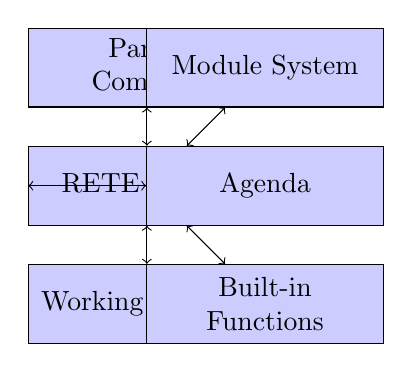
\begin{tikzpicture}[
  node distance=1.5cm and 2cm,
  component/.style={rectangle, draw, fill=blue!20, minimum width=3cm, minimum height=1cm, align=center}
]
  \node[component] (parser) {Parser \\ Compiler};
  \node[component, below of=parser] (rete) {RETE Engine};
  \node[component, below of=rete] (wm) {Working Memory};
  \node[component, right of=rete] (agenda) {Agenda};
  \node[component, above of=agenda] (modules) {Module System};
  \node[component, below of=agenda] (functions) {Built-in \\ Functions};
  
  \draw[<->] (parser) -- (rete);
  \draw[<->] (rete) -- (wm);
  \draw[<->] (rete) -- (agenda);
  \draw[<->] (modules) -- (rete);
  \draw[<->] (functions) -- (rete);
\end{tikzpicture}
\caption{Architettura CLIPS ad alto livello}
\end{figure}

\subsection{Flusso di Esecuzione}

\begin{algorithm}
\caption{Ciclo Principale CLIPS}
\begin{algorithmic}[1]
\Function{CLIPSMainLoop}{}
  \State \Call{InitializeEnvironment}{}
  \State \Call{LoadRules}{rulefile}
  \State \Call{Reset}{}
  \While{not halted}
    \State \Comment{Recognize phase}
    \State $conflictSet \gets $ \Call{UpdateRETENetwork}{}
    \If{$conflictSet = \emptyset$}
      \State break \Comment{Quiescence}
    \EndIf
    \State \Comment{Act phase}
    \State $activation \gets $ \Call{SelectFromAgenda}{$conflictSet$}
    \State \Call{FireRule}{$activation$}
  \EndWhile
\EndFunction
\end{algorithmic}
\end{algorithm}

\section{Costrutti del Linguaggio}

\subsection{Deftemplate}

Definiscono struttura dei fatti:

\begin{lstlisting}[language=CLIPS]
(deftemplate persona
  "Template per rappresentare una persona"
  (slot nome (type STRING))
  (slot eta (type INTEGER) (range 0 150))
  (slot professione (default "disoccupato"))
  (multislot hobby (allowed-values sport lettura cinema)))
\end{lstlisting}

\subsection{Defrule}

Regole di produzione:

\begin{lstlisting}[language=CLIPS]
(defrule promuovi-senior
  "Promuove impiegati con esperienza"
  (declare (salience 10))
  (impiegato (id ?id) (anni-servizio ?a&:(>= ?a 10)))
  (not (promosso ?id))
  =>
  (assert (promosso ?id))
  (printout t "Promosso impiegato " ?id crlf))
\end{lstlisting}

\subsection{Deffacts}

Fatti iniziali:

\begin{lstlisting}[language=CLIPS]
(deffacts stato-iniziale
  "Popolazione iniziale working memory"
  (impiegato (id 1) (nome "Mario") (anni-servizio 12))
  (impiegato (id 2) (nome "Giulia") (anni-servizio 5)))
\end{lstlisting}

\subsection{Defmodule}

Organizzazione in moduli:

\begin{lstlisting}[language=CLIPS]
(defmodule ACQUISIZIONE
  "Modulo per input dati"
  (export deftemplate persona ordine))

(defmodule ELABORAZIONE
  "Modulo per business logic"
  (import ACQUISIZIONE deftemplate persona ordine))
\end{lstlisting}

\section{Struttura Interna}

\subsection{Environment}

Contesto isolato di esecuzione:

\begin{lstlisting}[language=C]
struct environment {
    struct fact *factList;
    struct defrule *ruleList;
    struct defmodule *moduleList;
    struct agenda *currentAgenda;
    struct partialMatch *betaMemory;
    // ... molti altri campi
};
\end{lstlisting}

\textbf{Supporto multi-environment}: Permette instanze CLIPS separate.

\subsection{Fact Management}

\begin{lstlisting}[language=C]
struct fact {
    struct factHeader header;
    struct deftemplate *whichDeftemplate;
    unsigned long factIndex;
    struct multifield *theProposition;
    struct fact *previousFact;
    struct fact *nextFact;
};
\end{lstlisting}

\subsection{Rule Structure}

\begin{lstlisting}[language=C]
struct defrule {
    struct constructHeader header;
    int salience;
    int localVarCnt;
    struct expr *dynamicSalience;
    struct defruleModule *header.whichModule;
    struct joinNode *lastJoin;
    struct expr *actions;
    // ...
};
\end{lstlisting}

\section{Gestione della Memoria}

\subsection{Memory Pool}

CLIPS usa pool di memoria per efficienza:

\begin{lstlisting}[language=C]
struct memoryPtr {
    struct memoryPtr *next;
};

void *RequestChunk(unsigned int size) {
    if (TopMemoryBlock != NULL) {
        struct memoryPtr *theMemory = TopMemoryBlock;
        TopMemoryBlock = theMemory->next;
        return (void *) theMemory;
    }
    return malloc(size);
}

void ReturnChunk(void *ptr, unsigned int size) {
    struct memoryPtr *theMemory = (struct memoryPtr *) ptr;
    theMemory->next = TopMemoryBlock;
    TopMemoryBlock = theMemory;
}
\end{lstlisting}

\textbf{Beneficio}: Riduzione chiamate malloc/free, meno frammentazione.

\section{I/O e Router System}

\subsection{Router}

Meccanismo flessibile per I/O:

\begin{lstlisting}[language=C]
struct router {
    char *name;
    int priority;
    int (*query)(char *, char *);
    int (*print)(char *, char *);
    int (*getc)(char *);
    int (*ungetc)(int, char *);
    int (*exit)(int);
    struct router *next;
};
\end{lstlisting}

\textbf{Usi}:
\begin{itemize}
\item Redirigere output a file/GUI
\item Interceptare comandi
\item Logging e debugging
\item Integrazione con applicazioni
\end{itemize}

\section{Estensibilità}

\subsection{User-Defined Functions (UDF)}

\begin{lstlisting}[language=C]
#include "clips.h"

void MyFunction(Environment *env, UDFContext *context, UDFValue *ret) {
    UDFValue arg1, arg2;
    
    UDFNthArgument(context, 1, NUMBER_TYPES, &arg1);
    UDFNthArgument(context, 2, NUMBER_TYPES, &arg2);
    
    ret->integerValue = CreateInteger(env, 
        arg1.integerValue->contents + arg2.integerValue->contents);
}

int main() {
    Environment *env = CreateEnvironment();
    AddUDF(env, "my-add", "l", 2, 2, "ll", MyFunction, "MyFunction", NULL);
    // ...
}
\end{lstlisting}

\subsection{External Calls}

Chiamare funzioni esterne da regole:

\begin{lstlisting}[language=CLIPS]
(defrule call-external
  (trigger)
  =>
  (bind ?result (my-add 10 20))
  (printout t "Result: " ?result crlf))
\end{lstlisting}

\section{Debugging e Profiling}

\subsection{Watch Facilities}

\begin{lstlisting}[language=CLIPS]
(watch facts)           ; Trace assert/retract
(watch rules)           ; Trace rule firing
(watch activations)     ; Trace agenda changes
(watch compilations)    ; Trace parsing
\end{lstlisting}

\subsection{Comandi Diagnostici}

\begin{lstlisting}[language=CLIPS]
(facts)                 ; Lista tutti i fatti
(rules)                 ; Lista tutte le regole
(agenda)                ; Mostra conflict set
(matches rule-name)     ; Mostra partial match
\end{lstlisting}

\section{Performance}

\subsection{Ottimizzazioni Interne}

\begin{itemize}
\item \textbf{Incremental reset}: Reset parziale
\item \textbf{Dynamic salience}: Calcolo lazy
\item \textbf{Pattern indexing}: Hash su pattern comuni
\item \textbf{Join network sharing}: Riuso nodi
\item \textbf{Memory compaction}: Garbage collection periodica
\end{itemize}

\subsection{Benchmark Tipici}

\begin{table}[h]
\centering
\begin{tabular}{@{}lrr@{}}
\toprule
\textbf{Sistema} & \textbf{Regole} & \textbf{Cicli/sec} \\
\midrule
Piccolo & 10-100 & 10000+ \\
Medio & 100-1000 & 1000-5000 \\
Grande & 1000+ & 100-1000 \\
\bottomrule
\end{tabular}
\caption{Performance indicative CLIPS}
\end{table}

\section{Integrazione con Applicazioni}

\subsection{Embed CLIPS}

\begin{lstlisting}[language=C]
#include "clips.h"

int main(int argc, char *argv[]) {
    Environment *env = CreateEnvironment();
    
    // Carica regole
    Load(env, "rules.clp");
    Reset(env);
    
    // Assert fatti da applicazione
    AssertString(env, "(temperatura 25)");
    
    // Esegui inference
    Run(env, -1);
    
    // Interroga risultati
    Eval(env, "(find-all-facts ((?f risultato)) TRUE)", &result);
    
    DestroyEnvironment(env);
    return 0;
}
\end{lstlisting}

\subsection{Callback}

Notifiche da CLIPS ad applicazione:

\begin{lstlisting}[language=C]
bool RuleFireCallback(
    Environment *env,
    Defrule *rule,
    void *context
) {
    printf("Fired: %s\n", DefruleName(rule));
    return true;  // Continue execution
}

AddRunFunction(env, "my-callback", RuleFireCallback, 0, NULL);
\end{lstlisting}

\section{Conclusioni del Capitolo}

\subsection{Punti Chiave}

\begin{enumerate}
\item CLIPS è un sistema \textbf{maturo e collaudato} (35+ anni)
\item Architettura \textbf{modulare ed estensibile}
\item Efficienza grazie a \textbf{RETE ottimizzato}
\item \textbf{Portabilità} eccellente (C standard)
\item Supporto completo per \textbf{sviluppo enterprise}
\end{enumerate}

\subsection{Prossimi Capitoli}

\begin{itemize}
\item Cap.~\ref{cap:clips_strutture}: Strutture dati interne dettagliate
\item Cap.~\ref{cap:clips_memoria}: Gestione memoria
\item Cap.~\ref{cap:clips_agenda}: Sistema di agenda e conflict resolution
\item Cap.~\ref{cap:clips_moduli}: Sistema di moduli e namespace
\end{itemize}

\subsection{Letture Consigliate}

\begin{itemize}
\item CLIPS Reference Manual (6.4)
\item CLIPS Architecture Manual
\item Giarratano \& Riley (2004). "Expert Systems: Principles and Programming"
\item Riley, G. (2016). "CLIPS: A Tool for Building Expert Systems"
\end{itemize}
